
\begin{center}
    \textbf{\fontsize{20}{22}\selectfont  III: KẾT LUẬN VÀ ĐÁNH GIÁ}
\end{center}

\noindent\textbf{\fontsize{16}{20}\selectfont 3.1. Hệ thống thu thập, lưu trữ}

Hình~\ref{fig:mach} là kết quả mạch đã hoàn thiện. Để đánh giá mạch hoạt động
ổn định, tác ra tiến hành đo kiểm điện áp đầu vào và điện áp đầu ra của bộ hạ
áp, chân kết nối cảm biến, dữ liệu trả về.

\begin{figure}[H]
    \centering
    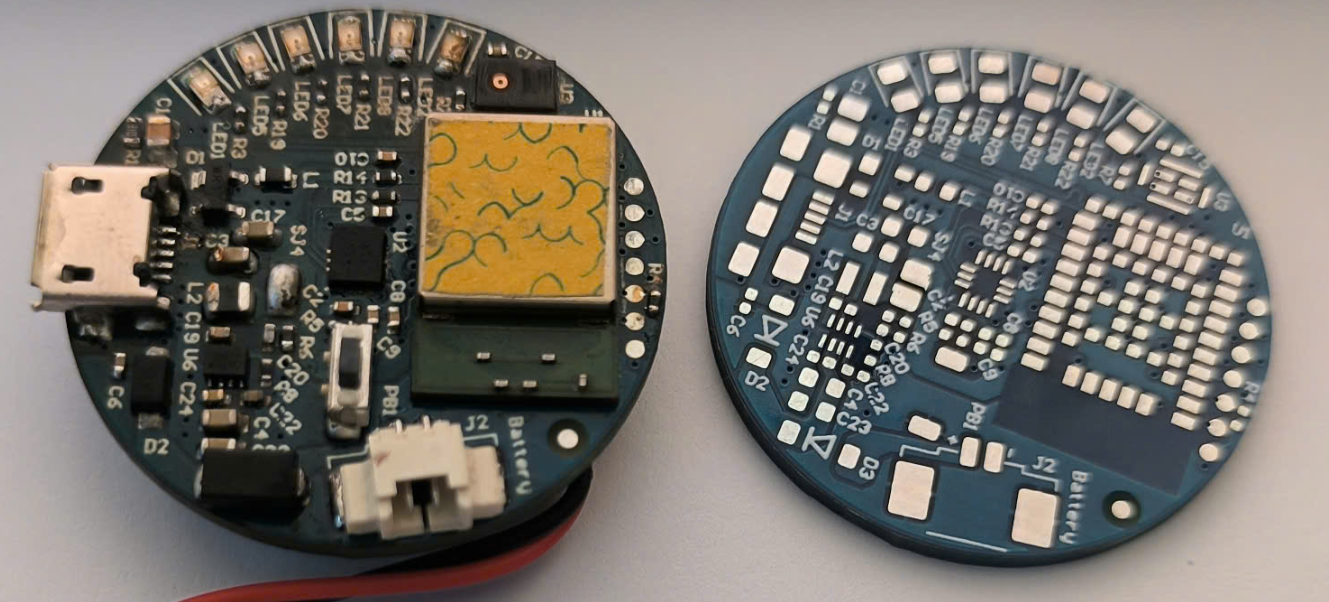
\includegraphics[width=0.5\textwidth]{images/mach.png}
    \caption{Mạch hoàn chỉnh}
    \label{fig:mach}
\end{figure}

\begin{figure}[H]
    \centering
    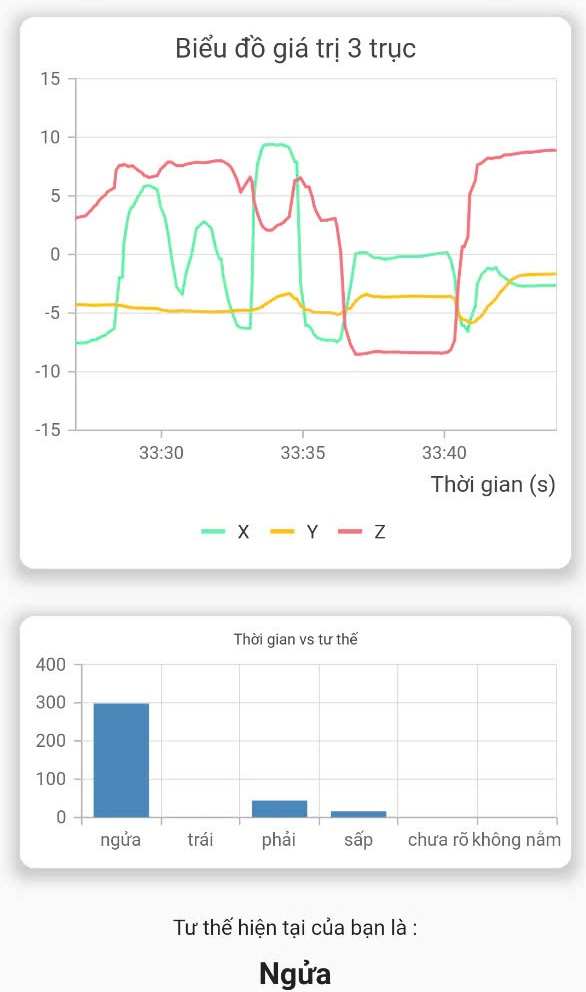
\includegraphics[width=0.3\linewidth]{images/ketqua_bieudoxyz.jpg}
    \caption{Màn hình hiển thị dữ liệu gia tốc ba trục với trục hoàng là giá trị thời gian, trục tung là giá trị cảm biến gấp lên 10 lần }
    \label{ketqua_bieudoxyz}
\end{figure}

\noindent\textbf{\fontsize{16}{20}\selectfont 3.2. Thu thập và gắn nhãn dữ liệu}

Tổng cộng 25 tình nguyện viên đã được tuyển chọn tham gia vào quá trình thu
thập dữ liệu, với độ tuổi dao động từ 10 đến 60, trong đó độ tuổi phổ biến là
24. Nhóm tình nguyện viên bao gồm cả nam và nữ, được lựa chọn với tiêu chí đa
dạng về giới tính và độ tuổi nhằm tăng tính đại diện và khách quan cho bộ dữ
liệu.
\begin{figure}[H]
    \centerline{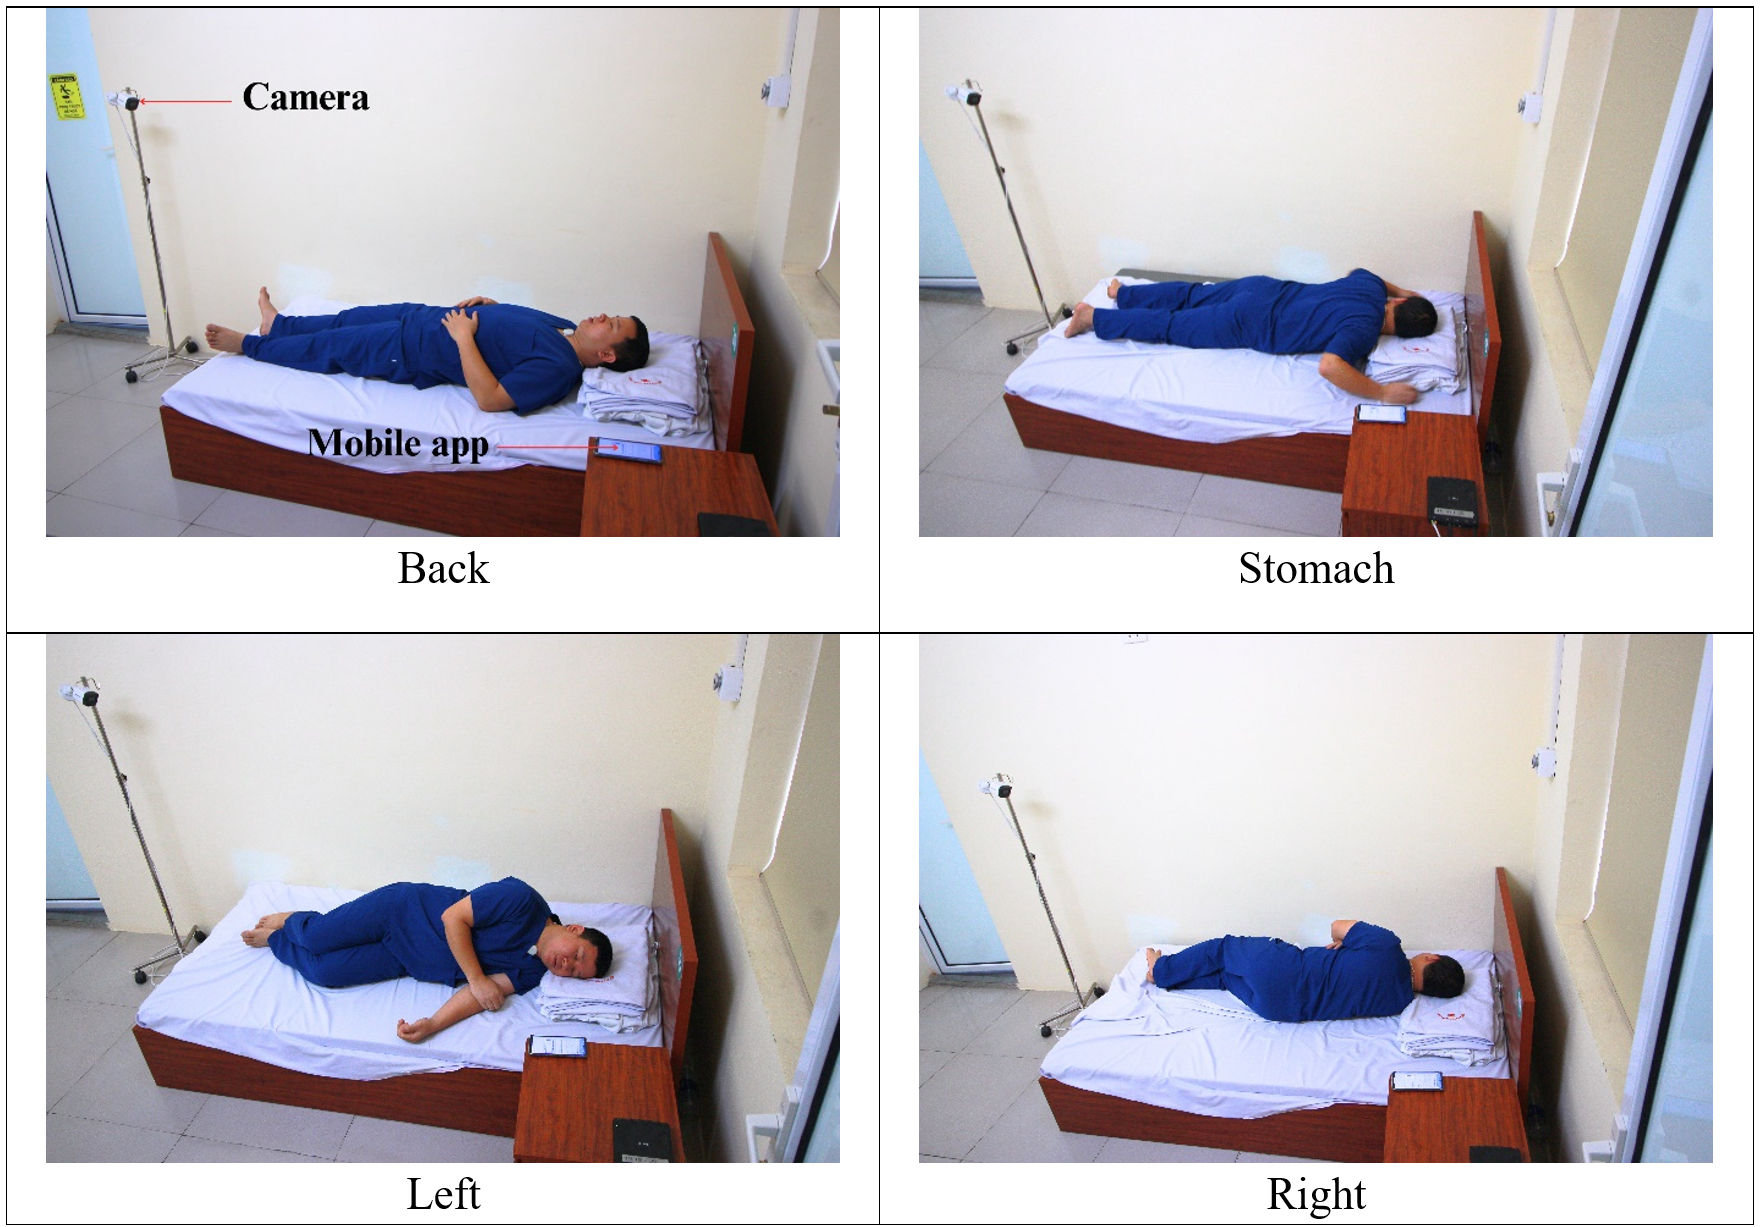
\includegraphics[width=0.8\linewidth]{images/4position.png}}
    \caption{Mô phỏng thực nghiệm thực tế}
    \label{4Position}
\end{figure}

Trong kịch bản đầu tiên (gọi là thu thập có giám sát), mỗi tình nguyện viên
được hướng dẫn gắn thiết bị dưới dự giám sát của nhóm. Bên cạnh đó, để mô phỏng
điều kiện thực tế khi sử dụng thiết bị trong khi ngủ ban đêm, hiện kịch bản thứ
hai (gọi là thu thập trong giấc ngủ tự nhiên) được xây dựng.

\noindent\textbf{\fontsize{16}{20}\selectfont 3.3. Phân loại tư thế ngủ bằng học máy}

\noindent\textbf{\fontsize{14}{5}\selectfont 3.3.1. Phân tích dữ liệu}

Hình~\ref{fig:ana_balance} cho thấy phân bố dữ liệu của tập huấn luyện tương
đối cân bằng. Còn đối với tập kiểm thử, tư thế nằm ngửa và nghiêng trái chiếm
đa số. Những lập luận trên hoàn toàn đúng với bài toán học máy phân loại tư thế
ngủ bởi vì: trên bộ huấn luyện, các nhãn cần được giữ ở mức cân bằng để tránh
tình trạng quá khớp; còn trên tập kiểm thử, các nhãn sẽ có xu hướng phản ánh
đúng sinh lý của cá nhân khi ngủ, sẽ thường có những tư thế nổi bật hẳn về số
lượng do thói quen.

\begin{figure}[H]
    \centering
    \begin{subfigure}[b]{0.48\textwidth}
        \centering
        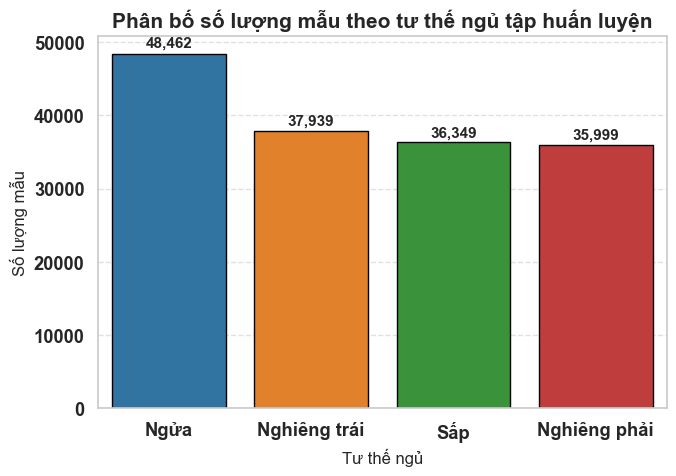
\includegraphics[width=1\textwidth]{images/ana_balance_train.png}
        \label{fig:ana_balance_train}

    \end{subfigure}
    \begin{subfigure}[b]{0.48\textwidth}
        \centering
        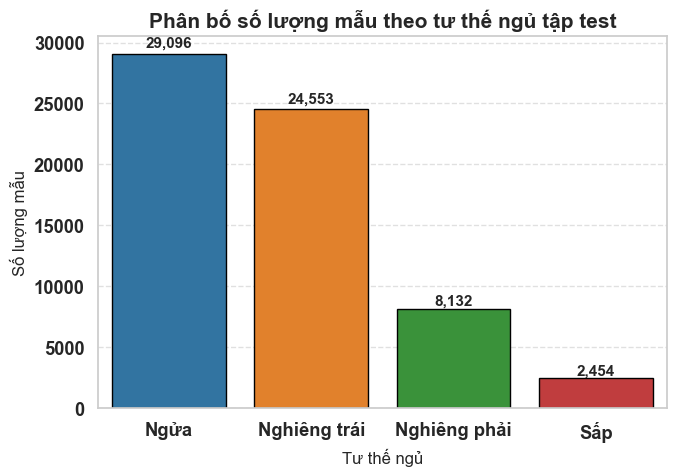
\includegraphics[width=1\textwidth]{images/ana_balance_test.png}
        \label{fig:ana_balance_test}
    \end{subfigure}
    \caption{Biểu đồ phân bố các nhãn thu được}
    \label{fig:ana_balance}
\end{figure}

Luận văn có trình bày chi tiết về những nhận định đưa ra về phân bố giá trị các
trục x, y, z đối với bài toán tư thế ngủ. Trục x, z sẽ chiến nhiều ý nghĩa đối
với việc đánh giá hơn trục y.

\begin{figure}[H]
    \centering
    \begin{subfigure}[b]{0.48\textwidth}
        \centering
        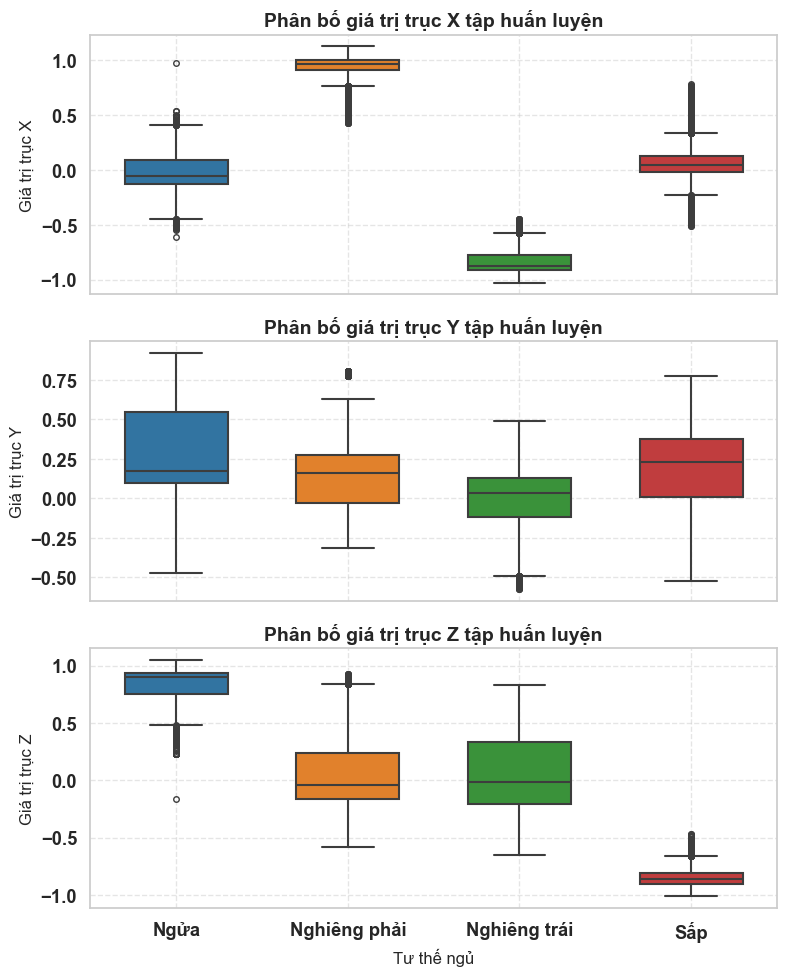
\includegraphics[width=1\textwidth]{images/ana_distribute_train.png}
        \label{fig:ana_distribute_train}
        \caption{tập huấn luyện}
    \end{subfigure}
    \begin{subfigure}[b]{0.48\textwidth}
        \centering
        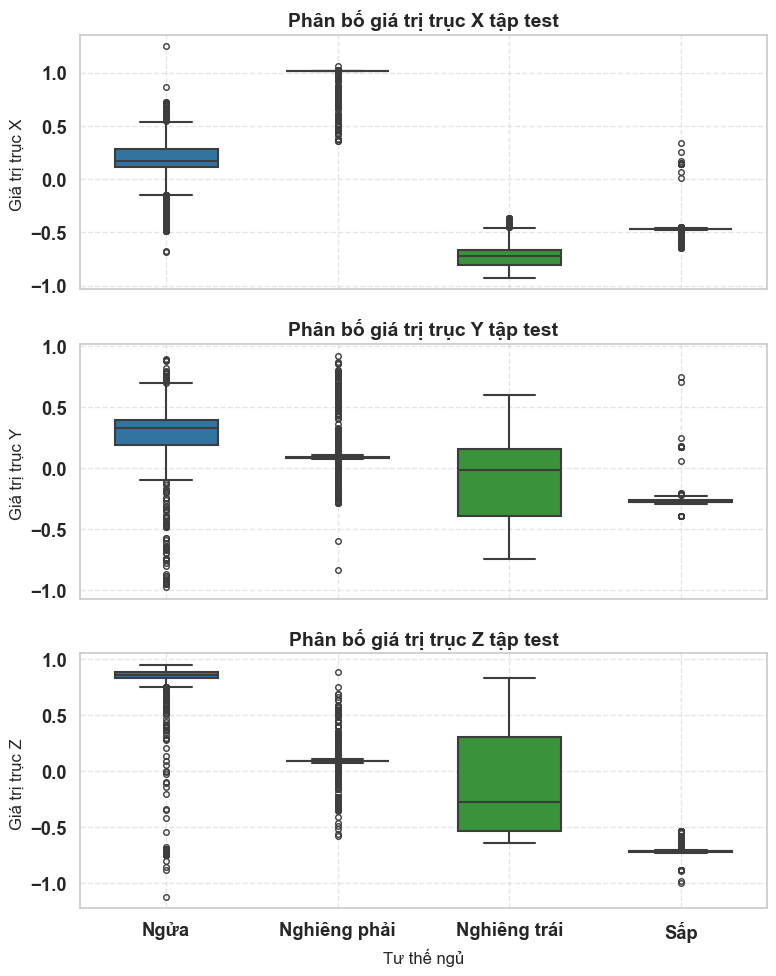
\includegraphics[width=1\textwidth]{images/ana_distribute_test.png}
        \label{fig:ana_distribute_test}
        \caption{tập kiểm thử}
    \end{subfigure}
    \caption{Biểu đồ phân bố dữ liệu 3 trục theo các tư thế ngủ}
    \label{fig:ana_distribute}
\end{figure}

\noindent\textbf{\fontsize{14}{5}\selectfont 3.3.2. Xử lý và trích xuất đặc trưng}

Dữ liệu cảm biến thu thập được trước tiên được xử lý khử nhiễu bằng phương pháp
hiệu chỉnh điểm gốc, bằng cách lấy hiệu giữa giá trị hiện tại và giá trị tham
chiếu ban đầu trên ba trục $x$, $y$, $z$. Sau đó, tín hiệu được chia thành các
cửa sổ thời gian có độ dài 2 giây, với mức chồng lấn 50\% giữa các cửa sổ. Chỉ
những cửa sổ dữ liệu có nhãn nhất quán trong toàn bộ thời gian mới được giữ lại
để huấn luyện mô hình. Các cửa sổ chứa nhãn không đồng nhất (nhiều hơn một
nhãn) hoặc có biểu hiện chuyển động bất thường sẽ bị loại bỏ khỏi quá trình xử
lý tiếp theo. Sau đó, trích xuất ra 40 đặc trưng miền thời gian và 29 đặc trưng
miền tần số.

Việc sử dụng đồng thời các đặc trưng từ cả hai miền thời gian và tần số giúp
tăng khả năng mô tả đặc trưng cho mô hình học máy, từ đó nâng cao hiệu quả phân
loại tư thế ngủ trong các điều kiện khác nhau.

\begin{figure}[htbp]
    \centerline{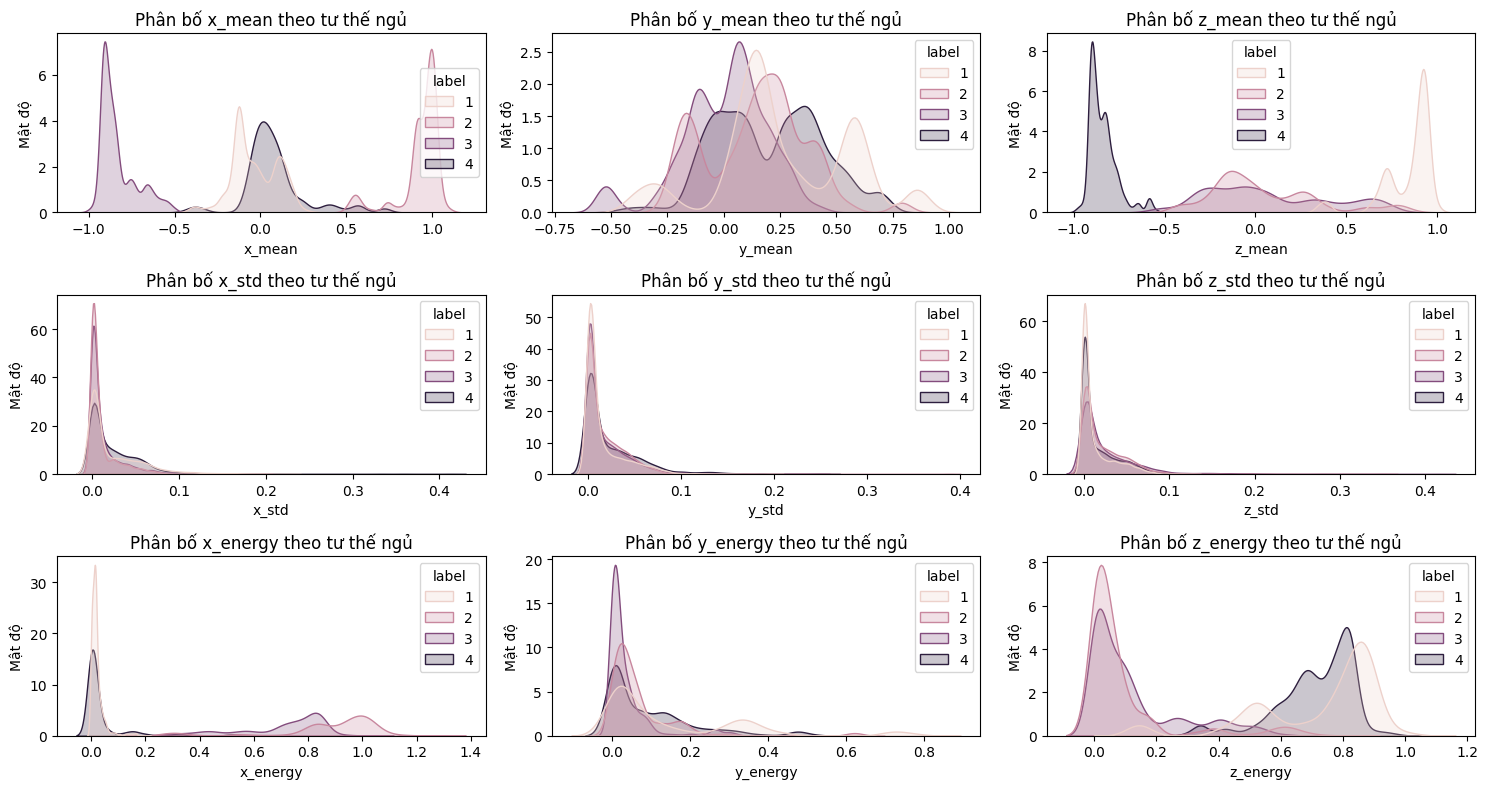
\includegraphics[width=1\linewidth]{images/ana_feature_time.png}}
    \caption{Phân bố của đặc trưng trung bình, độ lệnh chuẩn và năng lượng trên miền thời gian của tập huấn luyện}
    \label{ana_feature_time}
\end{figure}

Hình~\ref{ana_feature_time} minh họa phân bố của ba đặc trưng miền thời gian.
Các đặc trưng trung bình và năng lượng của 2 trục x và z cho phân bố mật độ
tách biệt để phân bật nhóm tư thế nghiêng trái - nghiêng phải và ngửa - sấp.
Đối với trục y, phân bố của các tư thế có xu hướng giống nhau và cũng tương tự
các đặc trưng độ lệnh chuẩn trên miền thời gian và các hai giá trị đặc trưng
trên miền tần số Hình~\ref{ana_feature_fft}.

\begin{figure}[H]
    \centerline{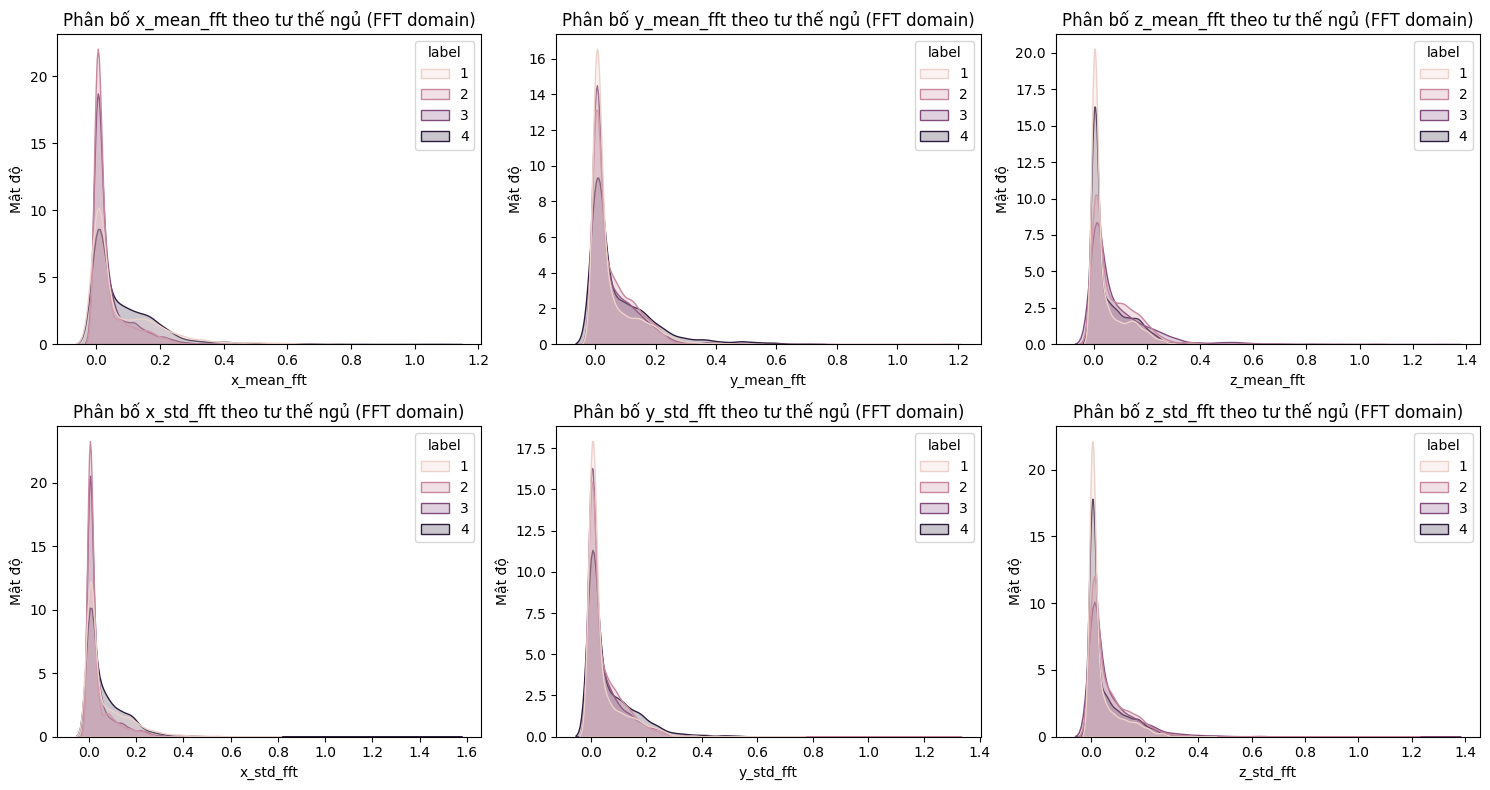
\includegraphics[width=1\linewidth]{images/ana_feature_fft.png}}
    \caption{Phân bố của đặc trưng trung bình, độ lệnh chuẩn trên miền tần số của tập huấn luyện}
    \label{ana_feature_fft}
\end{figure}

Qua phân tích trên, nhóm càng tin tưởng về luận điểm rằng với tư thế ngủ, các
đặc trưng miền thời gian sẽ có nhiều ý nghĩa hơn và trong đó cũng sẽ có những
nhóm thực sự nổi bật để có thể phân loại tư thế ngủ.

\noindent\textbf{\fontsize{14}{5}\selectfont 3.3.3. Lựa chọn tham số}

Sau khi xác định được 69 đặc trưng cả miền thời gian và tần số, các vòng lặp
với các dải tham số cài đặt sẵn trên 5 mô hình đã lựa chọn LR, RF, SVM, GB và
ANN sẽ được chạy thử nghiệm. Kết quả cho thấy mô hình RF và GB được đánh giá về
mặt độ chính xác là ổn định nhất cả quá trình xác thực chéo và tập kiểm tra.
Hai mô hình SVM và LR có độ chính xác thấp nhất trong 5 mô hình nhưng vẫn cho
độ chính xác > 94\%.

\begin{figure}[H]
    \centering
    \begin{subfigure}[b]{0.48\textwidth}
        \centering
        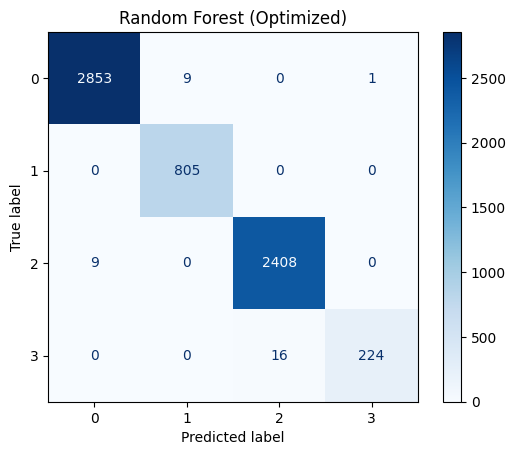
\includegraphics[width=0.8\textwidth]{images/ml_confuse_rf.png}
        \label{fig:ml_confuse_rf}
        \caption{RF}
    \end{subfigure}
    \begin{subfigure}[b]{0.48\textwidth}
        \centering
        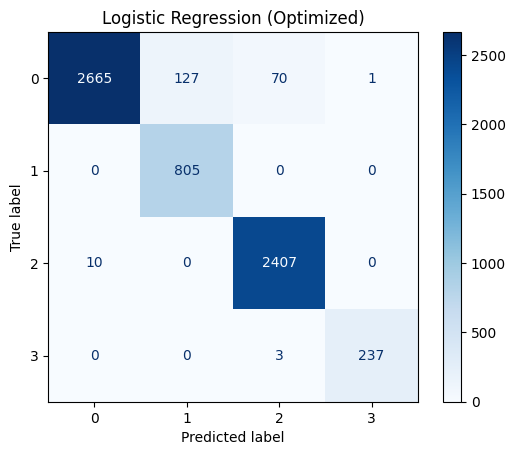
\includegraphics[width=0.8\textwidth]{images/ml_confuse_lr.png}
        \label{fig:ml_confuse_lr}
        \caption{LR}
    \end{subfigure}
    \begin{subfigure}[b]{0.48\textwidth}
        \centering
        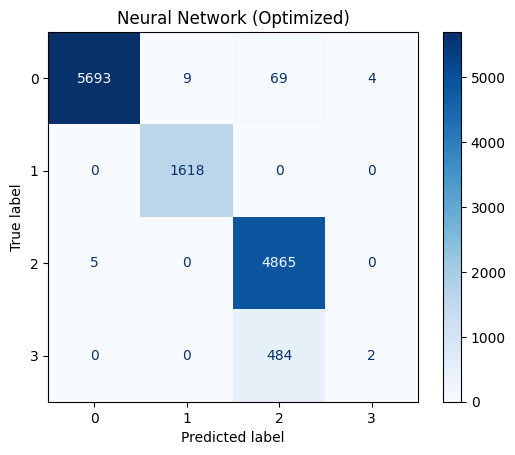
\includegraphics[width=0.8\textwidth]{images/ml_confuse_nn.png}
        \label{fig:ml_confuse_nn}
        \caption{ANN}
    \end{subfigure}
    \begin{subfigure}[b]{0.48\textwidth}
        \centering
        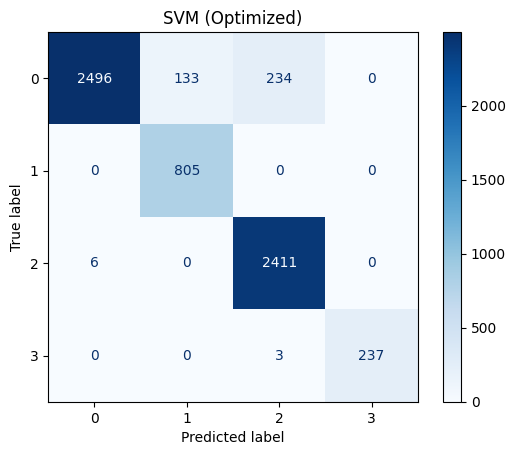
\includegraphics[width=0.8\textwidth]{images/ml_confuse_svm.png}
        \label{fig:ml_confuse_svm}
        \caption{SVM}
    \end{subfigure}
    \begin{subfigure}[b]{0.48\textwidth}
        \centering
        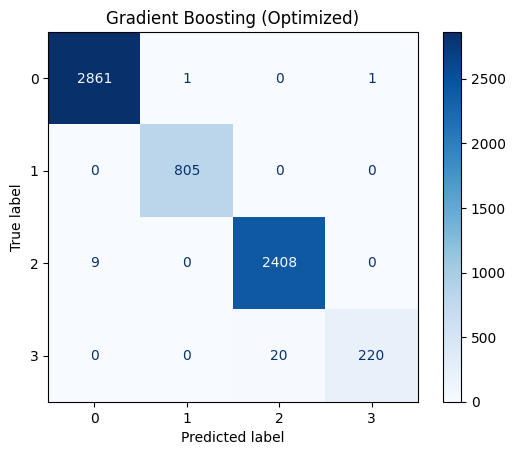
\includegraphics[width=0.8\textwidth]{images/ml_confuse_gb.png}
        \label{fig:ml_confuse_gb}
        \caption{GB}
    \end{subfigure}
    \caption{Ma trận nhầm lẫn của các mô hình}
    \caption*{\textit{Ghi chú:} Nhãn 0 - tư thế ngửa; 1 - nghiêng phải; 2 - nghiêng trái; 3 - sấp}
    \label{fig:ml_confuse}

\end{figure}
Để hiểu sâu hơn, trong khuôn khổ khóa luận sẽ tiến hành thêm các đánh giá về mức độ
ảnh hưởng của các đặc trưng
đến các mô hình (không có ANN vì lý do ANN không dùng 69
đặc trưng) Hình~\ref{fig:ml_shap}. Đúng với nhận định từ trước, các tính năng
miền thời gian chiếm nhiều ý nghĩa lên mô hình đặc biệt là đặc trưng được trích
xuất từ hai trục x, z và các đặc trưng tổng hợp từ 3 trục. Đặc trưng miền tần
số đa phần đứng vị trí cuối cho thấy không có nhiều ý nghĩa đối với các tham số
đã chọn.

\begin{figure}[H]
    \centering
    \begin{subfigure}[b]{0.48\textwidth}
        \centering
        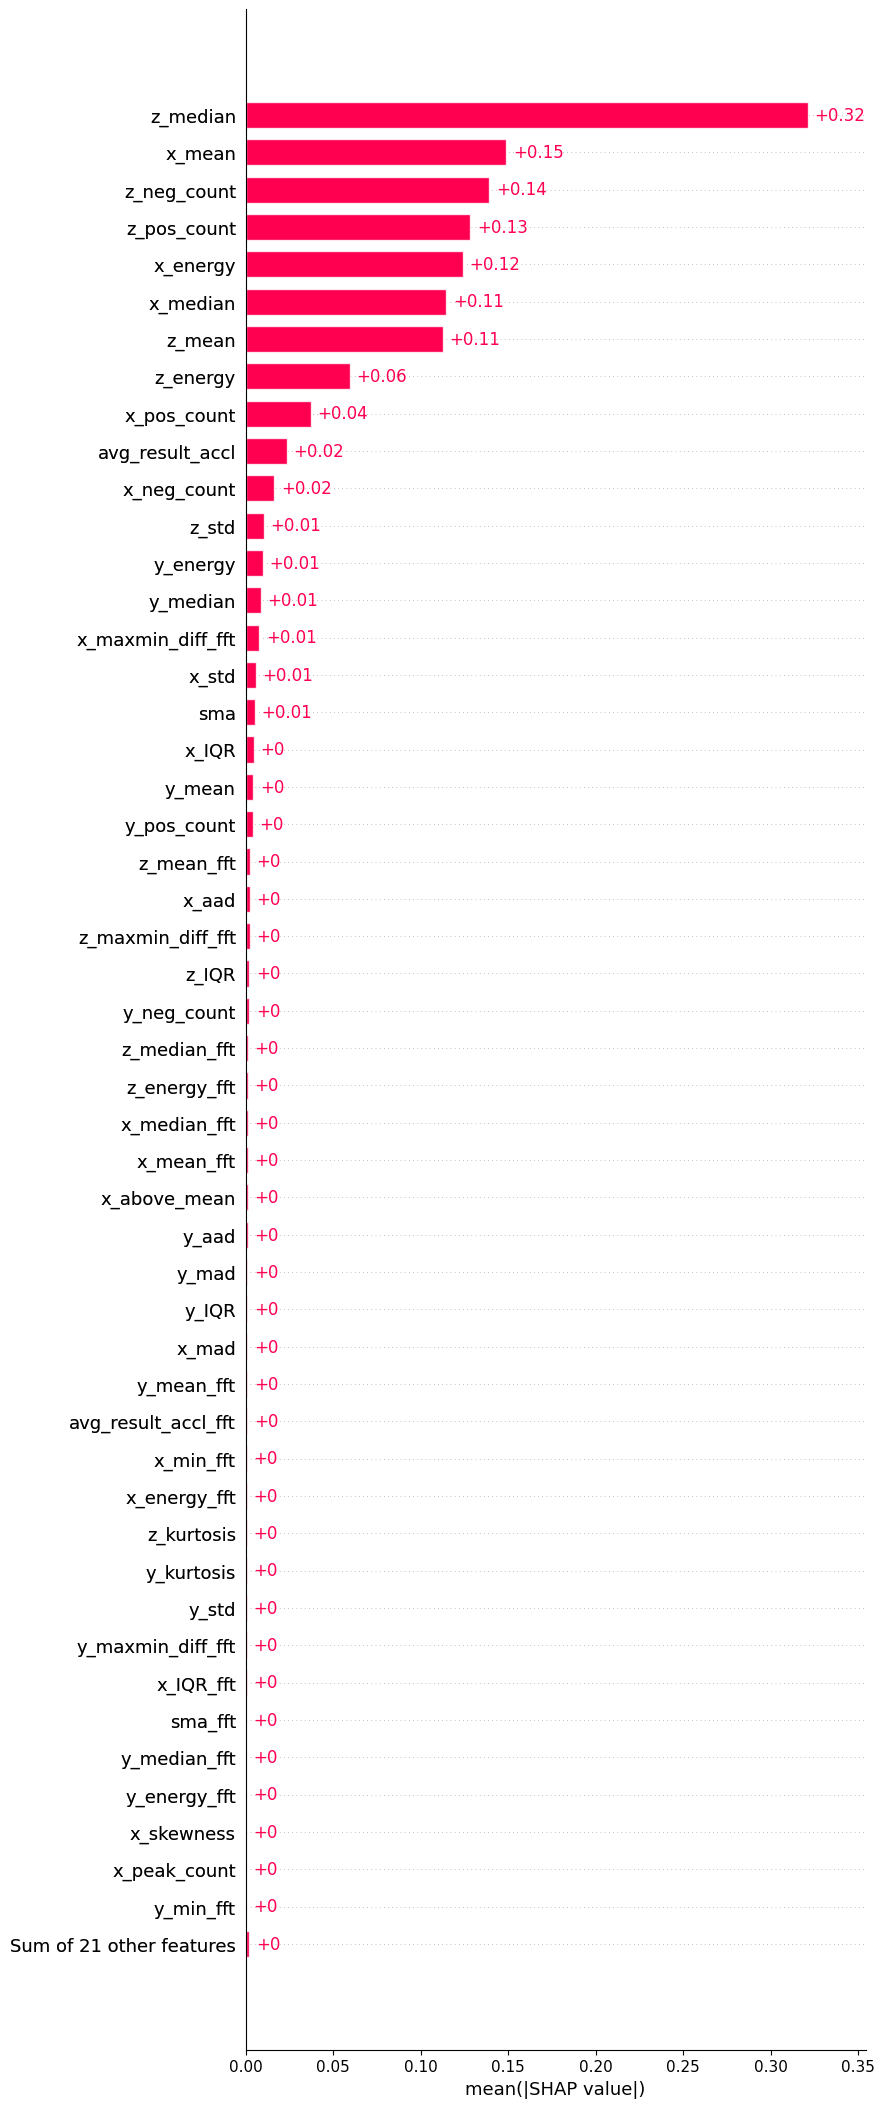
\includegraphics[width=0.6\textwidth]{images/ml_shap_rf.png}
        \label{fig:ml_shap_rf}
        \caption{RF}
    \end{subfigure}
    \begin{subfigure}[b]{0.48\textwidth}
        \centering
        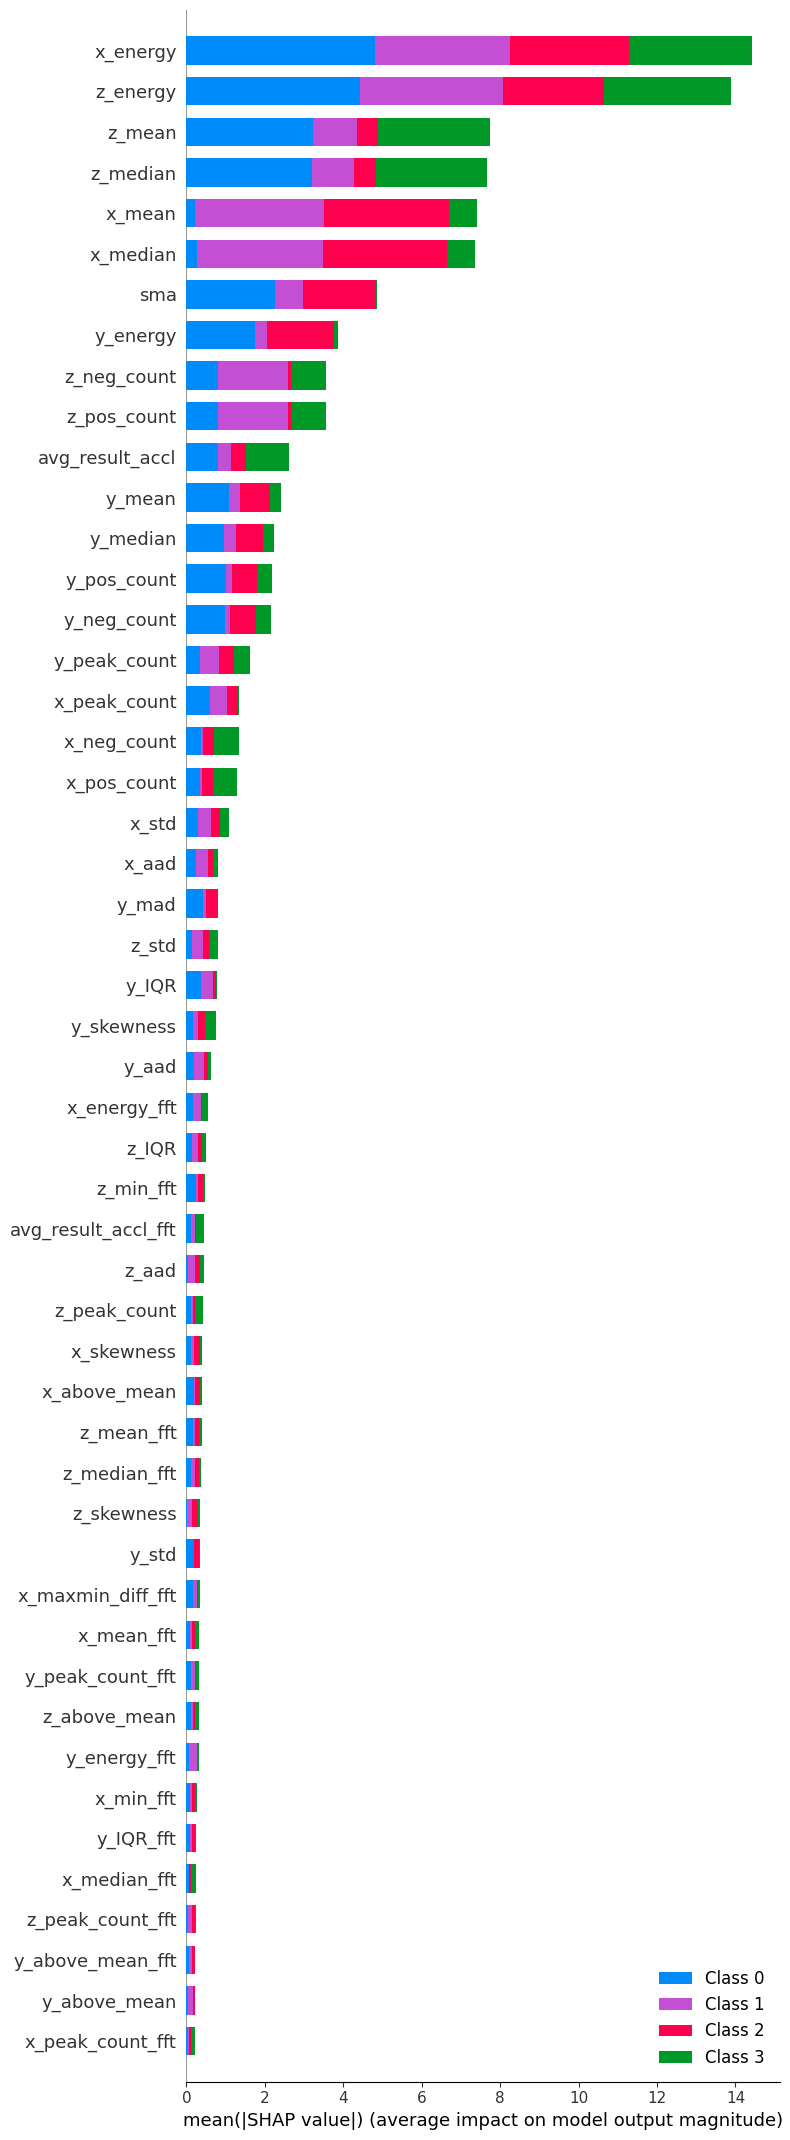
\includegraphics[width=0.5\textwidth]{images/ml_shap_lr.png}
        \label{fig:ml_shap_lr}
        \caption{LR}
    \end{subfigure}

    \begin{subfigure}[b]{0.48\textwidth}
        \centering
        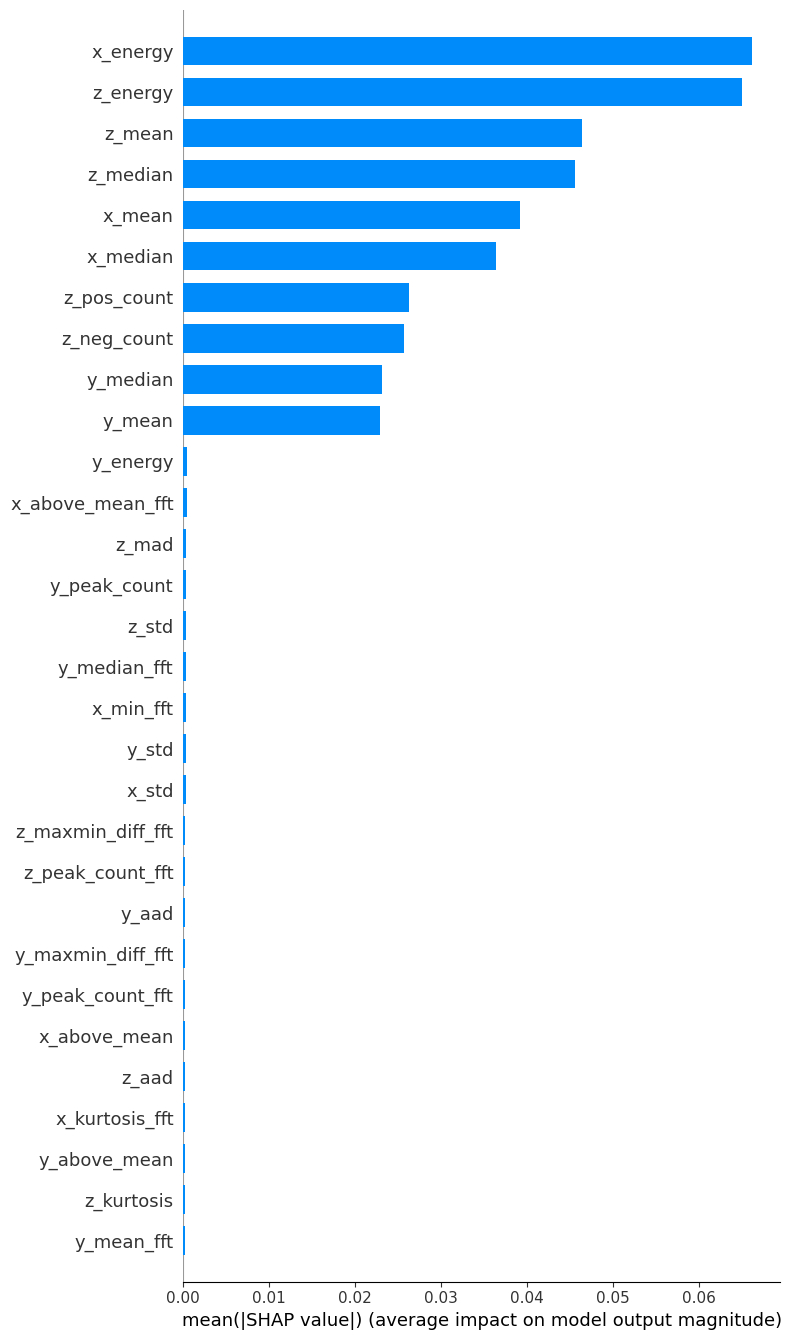
\includegraphics[width=0.5\textwidth]{images/ml_shap_svm.png}
        \label{fig:ml_shap_svm}
        \caption{SVM}
    \end{subfigure}
    \begin{subfigure}[b]{0.48\textwidth}
        \centering
        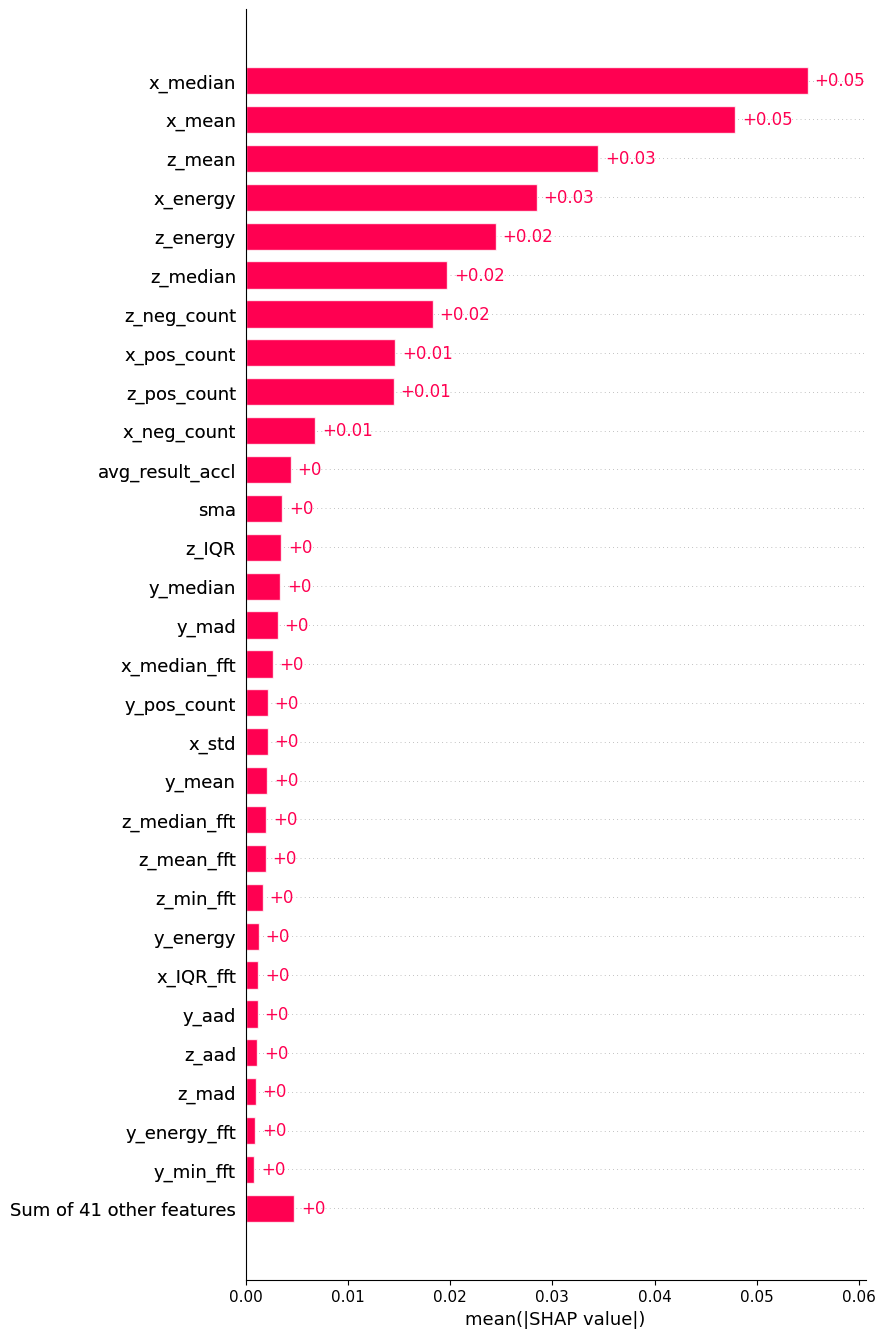
\includegraphics[width=0.6\textwidth]{images/ml_shap_gb.png}
        \label{fig:ml_shap_gb}
        \caption{GB}
    \end{subfigure}
    \caption{Ý nghĩa của các đặc trưng lên mô hình}
    \label{fig:ml_shap}

\end{figure}

Nhận thấy có 15 đặc trưng luôn xuất hiên vị trí đầu của tất cả các mô hình bao
gồm: 'z\_median', 'z\_mean', 'x\_mean', 'x\_energy', 'z\_pos\_count',
'z\_neg\_count', 'x\_median', 'z\_energy', 'avg\_result\_accl',
'x\_neg\_count', 'z\_std', 'x\_pos\_count', 'y\_energy', 'y\_mean', 'sma'. Để
hiểu sâu hơn về ý nghĩa các đặc trưng này, 8 kịch bản được xây dựng. Việc này
không chỉ có ý nghĩa về mặt phân tích đặc trưng và còn muốn làm rõ hơn về mặt
kích thước mô hình để phù hợp triển khai lên biên.

Kết hợp với phân tích ở phần trên, 3 thông số chính sẽ được thay đổi là: độ dài
cửa sổ - độ phủ, đặc trưng miền và số lượng đặc trưng Bảng~\ref{tab:scenarios}.

\begin{table}[H]
    \caption{Các kịch bản lựa chọn và sử dụng đặc trưng trong nghiên cứu}
    \label{tab:scenarios}
    \begin{center}
        \renewcommand{\arraystretch}{1.2}
        \begin{tabular}{|c|p{10cm}|}
            \hline
            \textbf{Kịch bản} & \textbf{Mô tả}                                                                                                \\
            \hline
            1                 & Dùng cửa sổ 20 mẫu (50\% độ phủ), với toàn bộ đặc trưng.                                                      \\
            \hline
            2                 & Dùng cửa sổ 20 mẫu (50\% độ phủ), với toàn bộ đặc trưng trong miền thời gian.                                 \\
            \hline
            3                 & Dùng cửa sổ 20 mẫu (50\% độ phủ), với toàn bộ đặc trưng trong miền tần số.                                    \\
            \hline
            4                 & Dùng cửa sổ 20 mẫu (50\% độ phủ), với đặc trưng miền thời gian, loại bỏ các đặc trưng có tương quan $>$ 95\%. \\
            \hline
            5                 & Dùng cửa sổ 20 mẫu (50\% độ phủ), với 15 đặc trưng quan trọng nhất theo giá trị đứng đầu.                     \\
            \hline
            6                 & Dùng cửa sổ 30 mẫu (50\% độ phủ), với 15 đặc trưng đứng đầu.                                                  \\
            \hline
            7                 & Dùng cửa sổ 10 mẫu (50\% độ phủ), với 15 đặc trưng đứng đầu.                                                  \\
            \hline
            8                 & Dùng cửa sổ 20 mẫu (25\% độ phủ), với 15 đặc trưng đứng đầu.                                                  \\
            \hline
        \end{tabular}
    \end{center}
\end{table}

\noindent\textbf{\fontsize{14}{5}\selectfont 3.3.4. Đánh giá kết quả}

Sau khi xác lập, tất cả các kịch bản sẽ tiến hành huấn luyện trên cũng một máy
tính và đưa ra kết quả về độ chính xác Hình~\ref{kq_8kb}.

Kết quả cho thấy, kịch bản 3 (màu đỏ) là toàn bộ các đặc trưng trên miền tần số
hoàn toàn không phù hợp để phân loại tư thế ngủ. Điều này cũng được chứng minh
tại ở phần trên. Các mô hình RF và GB luôn cho cho độ chính xác cao nhất và ổn
định nhất ở toàn bộ các bộ dữ liệu huấn luyện. Các kịch bản 5, 6, 7, 8 đựa trên
chỉ 15 đặc trưng (vị trí đầu), hầu như không thay đổi độ chính xác nhiều. Điều
này cho thấy, việc lựa chọn này phù hợp đối với bài toán tư thế ngủ. Trong kịch
bản 6, có độ chính xác cao nhất lên tới 99.84\% đối với mô hình GB với bộ dữ
liệu cửa sổ 30 mẫu. Kịch bản 7 có kết quả ấn tượng nhất với độ chính xác các mô
hình đều được cải thiện rõ rệt ngay cả mô hình LR và SVM. Điều này thực sự có ý
nghĩa vì độ rộng cửa sổ có ảnh hưởng trực tiếp đến việc tính toán, thời gian
phản hồi kết quả trên biên. Với ANN như đánh giá trong phần lựa chọn tham số,
khả năng tự trích xuất tính năng từ chỉ 2 lớp ẩn cũng đã cho kết quả đến 98\% ở
tập huấn luyện, nhưng giảm nhẹ ở tập kiểm tra 95.5\%.

\begin{figure}[htbp]
    \centerline{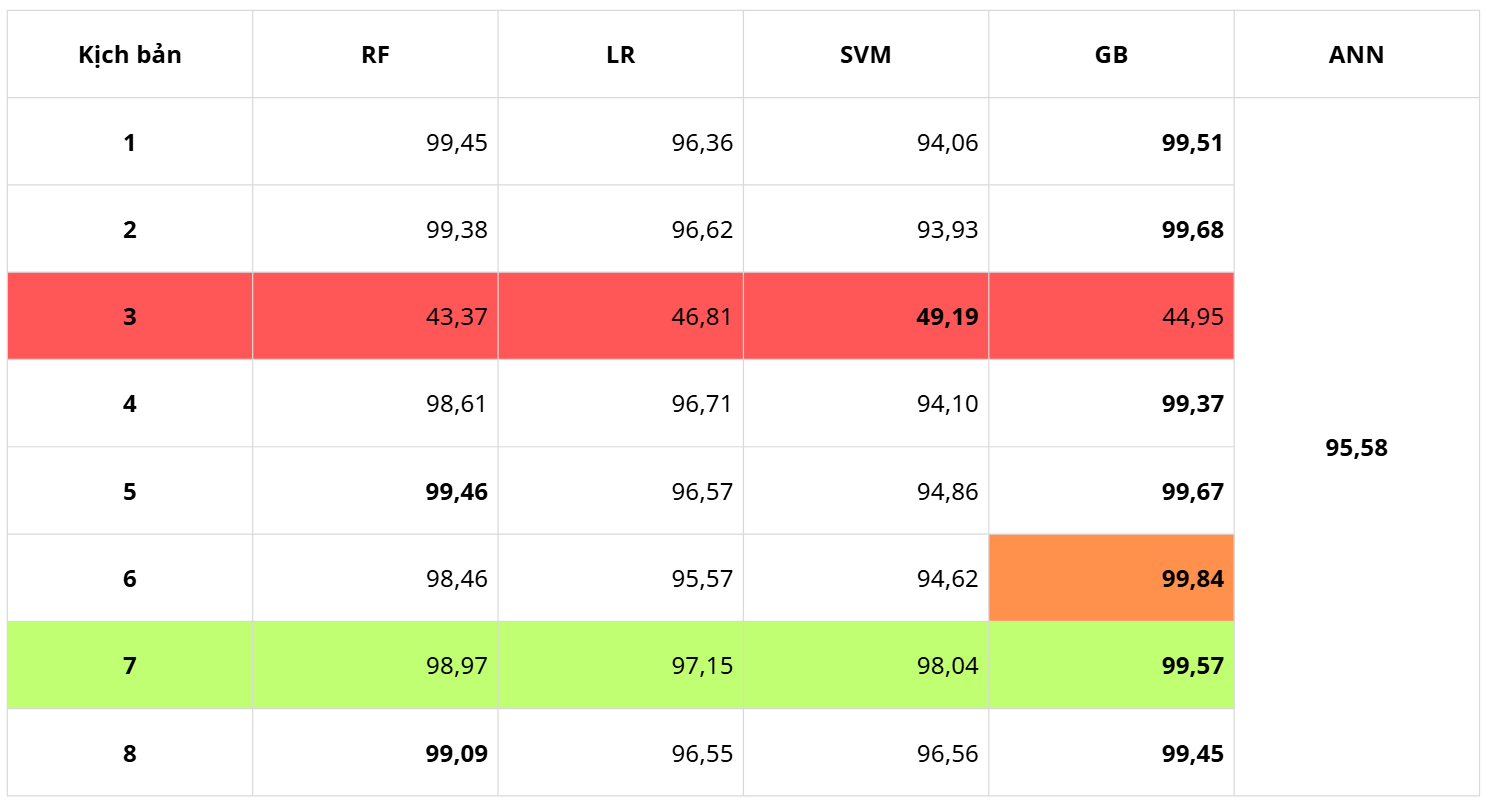
\includegraphics[width=1\linewidth]{images/kq_8kb.png}}
    \caption{Kết quả độ chính xác của 8 kịch bản}
    \label{kq_8kb}
\end{figure}

\begin{figure}[htbp]
    \centerline{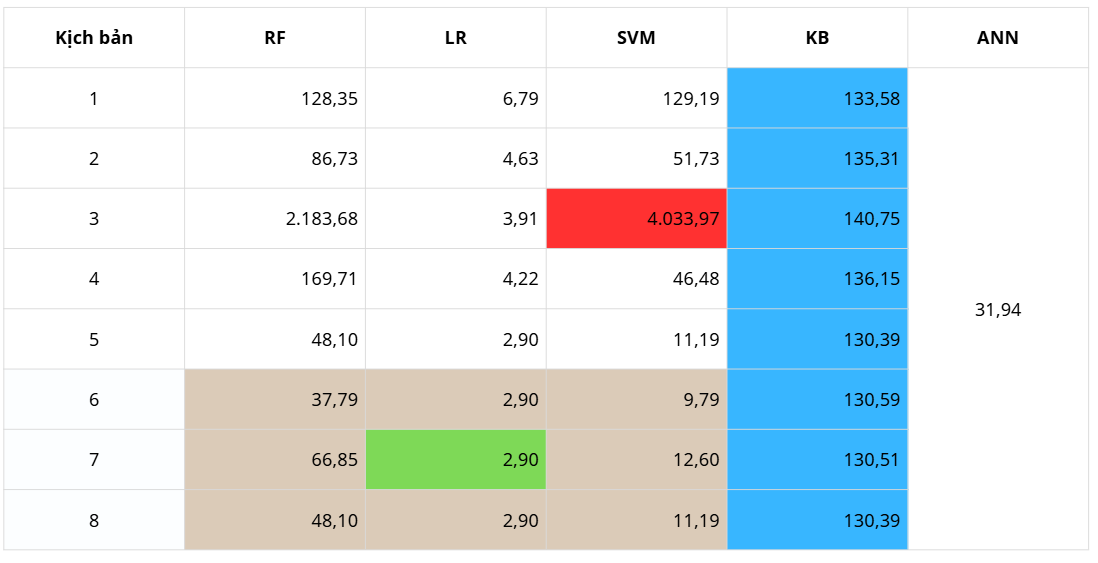
\includegraphics[width=1\linewidth]{images/kq_8kb_wei.png}}
    \caption{Kết quả kết thước mô hình của 8 kịch bản (đơn vị: kb)}
    \label{kq_8kb_wei}
\end{figure}

Hình~\ref{kq_8kb_wei} cho cái nhìn toàn diện về kích thước mô hình của 8 kịch
bản. Đầu tiên dễ nhận thấy là ở kịch bản 3, hai mô hình RF và SVM không hội tụ
được với bộ tham số đã tìm ra dẫn đến kích thước mô hình tăng vọt. Mô hình GB
có kích thước hầu như không thay đổi với tất cả kịch bản, nhưng luôn nằm trong
nhóm lớn nhất. Ở các kịch bản 5, 6, 7, 8 cũng thể hiện rõ giảm số lượng đặc
trưng không nhiều ý nghĩa xuống cũng đồng thời giảm được kích thước mô hình
nhưng độ chính xác hẫu như vẫn giữ nguyên. Dễ dàng nhìn thấy kịch bản thứ nhất
dùng tất cả các tính năng và kịch bản 7, tất cả kích thước mô hình ít nhất giảm
đi 2 lần, riêng SVM đạt tới 10 lần cho thấy việc lựa chọn đúng đặc trưng thực
sự có ý nghĩa mặt tính toán. Riêng đối với mô hình ANN, do chỉ đánh giá với 1
kịch bản nhưng cũng cho thấy tiềm năng mạnh mẽ khi chỉ với kích thước 31.94 kb
đã cho độ chính xác ở tập huấn luyện lên tới 98\%.

\noindent\textbf{\fontsize{16}{20}\selectfont 3.4. Triển khai mô hình lên phần cứng}

\noindent\textbf{\fontsize{14}{5}\selectfont 3.4.1. Chuyển đổi mô hình}

Phần này, luận văn sẽ trình bày các thức chuyển đổi từ mô hình được huấn luyện
trên máy tính về thành mô hình nhỏ gọn có thể triển khai tại biên.

\noindent\textbf{\fontsize{14}{5}\selectfont 3.4.2 Triển khai tại biên}
Phần này, luận văn sẽ trình bày sẽ thuật để đưa được mô hình đã chuyển đổi lên thiết bị phần cứng của nhóm.

\textbf{Đánh giá hiệu suất và tài nguyên}

Kết quả cho thấy LR có ưu thế vượt trội về tốc độ và mức tiêu thụ tài nguyên,
điều này khiến LR đặc biệt thích hợp cho các hệ thống nhúng giới hạn phần cứng
và yêu cầu phản hồi tức thời (ví dụ: phân loại tư thế ngủ). Tuy nhiên, ANN lại
có khả năng khai thác tốt hơn các quan hệ phi tuyến giữa dữ liệu cảm biến, giúp
tăng độ chính xác trong các bài toán phức tạp như nhận diện chuyển động liên
tục hoặc phân loại đa trạng thái.
\begin{table}[H]
    \centering
    \caption{So sánh hiệu năng LR và ANN trên nRF52840}
    \label{tab:comparison_full}
    \begin{tabular}{|l|p{5cm}|p{6cm}|}
        \hline
        \textbf{Tiêu chí}        & \textbf{Logistic Regression (LR)} & \textbf{Neural Network (ANN)} \\ \hline
        Dung lượng Flash sử dụng & 115,208 bytes (11\%)              & 363,520 bytes (36\%)          \\ \hline
        Dung lượng RAM sử dụng   & 46,632 bytes (17\%)               & 60,672 bytes (23\%)           \\ \hline
        Thời gian upload         & 4.9 s (29 pages)                  & 15 s (89 pages)               \\ \hline
        Thời gian suy luận       & 501~$\mu s$                       & 8000~$\mu s$                  \\ \hline
        Kích thước mô hình       & 2.9~kb                            & 23~kb                         \\ \hline

    \end{tabular}
\end{table}

Để đánh giá độ chính xác của 2 mô hình đã triển khai trên biên, một mô
hình có thể truyền toàn bộ dữ liệu tập kiểm
tra vào phần cứng và nhận lại giá trị suy luận được xây dựng.
Quy trình đánh giá mô hình trên vi điều khiển được tổ chức theo hai nhánh
chính: luồng xử lý trên MCU và luồng kiểm thử trên máy tính. Phía máy tính chịu
trách nhiệm tải dữ liệu gia tốc trong tệp CSV, tạo các cửa sổ trượt kích thước xác định. Tiếp đó, lần lượt truyền từng giá trị
(x,y,z) của mỗi cửa sổ xuống MCU thông qua giao tiếp Serial. Mỗi khi MCU nhận đủ
N mẫu, thiết bị thực thi toàn bộ pipeline suy luận gồm trích xuất 15 đặc trưng,
chuẩn hoá các đặc trưng theo min-max. Kết quả phân lớp từ phần cứng sẽ được trả về máy tính dưới dạng một số
nguyên đại diện cho tư thế ngủ.
Kết quả thực nghiệm cho thấy sự khác biệt rõ rệt giữa
Logistic Regression (LR) và mô hình Neural Network (ANN) khi đánh giá trên cùng
một tập dữ liệu gồm 12.749 cửa sổ tín hiệu. LR vẫn đạt độ chính xác 97.58\%,
trong khi ANN chỉ đạt 89.73\%. Sự chênh lệch này không chỉ phản ánh ưu thế của
LR trong điều kiện dữ liệu được chuẩn hóa tốt, mà còn làm nổi bật tính ổn định
của LR khi chuyển sang môi trường triển khai thực, vốn chứa nhiều bất định và
sai số đặc trưng của thiết bị biên.

\textbf{Bài toán phát hiện nằm hoặc không nằm}

Sau khi triển khai thực tế trên biên, có một vấn đề là hiện nay hệ thống tại
biên đang chỉ nhận dạng được 4 nhãn lần lượt ngửa, nghiêng phải, nghiêng trái,
sấp chưa đủ đáp ứng thực tế rằng khi ngủ người bệnh có thể đứng lên đi lại hoặc
uống nước. Qua đó, luận văn sẽ hướng tới mở rộng thêm bài toán xác định nằm hay
không nằm. Đây là bài toán sàng lọc trước khi đến bài toán xác định tư thế ngủ.
Để đạt được điều đó, 8,500 mẫu dữ liệu các hoạt động như ngồi, đi lại, uống
nước, được thu thập thêm. Tập các tư thế ngủ được chọn lọc tự tập dữ liệu huấn
luyện. Kết quả, 11,306 mẫu đủ các 4 tư thế được quy về 1 nhãn là nằm. Để thực
hiện bài toán phân loại ngủ hay không ngủ, toàn bộ các bước như đã trình bày
trong bài toán phân loại tư thế ngủ sẽ được áp dụng lại bao gồm: độ dài cửa sổ
1s, độ phủ 50\%, 69 đặc trưng trích xuất. Kết quả cho thấy, mô hình cho độ
chính xác lên tới 99.99\% phân loại 2 nhãn là nằm và không nằm và có kích thước
là 3.8 kb.

Sau khi đánh giá mức độ ảnh hưởng của đặc trưng lên mô hình, 6 đặc trưng:
'avg\_result\_accl', 'y\_energy', 'y\_min', 'y\_mean', 'z\_min', 'z\_max' được
chọn ra để huấn luyện lại mô hình LR. Kết quả độ chính xác có giảm 1 chút nhưng
kích thước mô hình còn 1.9 kb. Điều này hoàn toàn phù với tiêu chí để trải khai
đa mô hình trên biên.

Qua đó bài toán phân loại trên biên được nâng cấp thành 3 bước chính:

\usetikzlibrary{shapes.geometric, positioning}

\begin{tikzpicture}[node distance=20mm, >=latex]

    \node[draw] (data) {Dữ liệu cảm biến gia tốc};
    \node[draw, right=of data] (check) {Nằm hay không?};
    \node[draw, right=of check] (pose) {Tư thế ngủ};

    \draw[->] (data) -- (check);
    \draw[->] (check) -- node[above]{Có} (pose);
    \draw[->] (check) -- ++(0,-1.2) node[below]{Không};

\end{tikzpicture}

Việc này khẳng định để thực sự đưa bài toán này vào thực tế, còn rất nhiều bước
cần phải hiệu chỉnh để giải quyết các trường hợp thực tế. Tuy nhiên, các kết
quả đưa ra cho thấy giải quyết phần nào bài toán phân loại tư thế ngủ tại biên
cùng với 1 quy trình từ cảm biến đến mô hình trên biên.